\newpage
\section{Theoretische Grundlagen}


\subsection{Zielsetzung}
Das Ziel dieses Versuchs ist die Ausmessung eines Plexiglasquaders und eines Plastikauges mit Hilfe eines Ultraschallechoskop. 
Dabei soll ein grundlegendes Verständnis vom Umgang mit dem Echoskop vermittelt werden.

\subsection{Ultraschall}

\noindent
Der Mensch ist in der Lage Schall im Frequenzintervall von $\SI{16}{\hertz}$ bis $\SI{20}{\kilo\hertz}$ zu hören. 
Für den Menschen nicht hörbar ist dabei unter anderem der Ultraschall. 
Der Begriff ist für das Intervall von $\SI{20}{\kilo\hertz}$ bis $\SI{1}{\giga\hertz}$ definiert.\\
Darüber liegt der Hyperschall und unter dem hörbaren der Infraschall.\\
Ultraschall wird genutzt weren um Werkstücke oder menschliche Körper, ohne Schaden zu verursachen, zu untersuchen.\\\\

\noindent
Mathematisch lässt sich Schall durch eine longitudinal Welle ausdrücken:
\begin{equation*}
    p(x,t)=p_0+v_0\cdot Z\cdot \cos{(\omega t-kx)}
\end{equation*}
Der Term $Z=c\cdot \rho$ entspricht dabei der akustischen Impedanz, mit $\rho$ als Dichte des Mediums und $c$ der Schallgeschwindigkeit in dem Medium.\\
Die Schallgeschwindigkit hängt hierbei, da bei Schall Dichteänderungen auftreten, sehr stark vom Material ab.\\
In einer Flüssigkeit führt das mit der Kompressibilität $\kappa$ zu folgender Gleichung:
\begin{equation*}
    c_{Fl}=\sqrt{\frac{1}{\kappa\cdot\rho}}
\end{equation*}
In einem Festkörper verhällt sich das Ganze etwas anders. 
Dort zieht eine longitudinale Auslenkung von Teilchen, auf Grund der Rückstellkräfte, auch eine transversale Auslenkung nach sich.\\
Die Geschwindigkeit der beiden Ausbreitungsrichtungen variiert dabei.\\
Für den Festkörper muss dann $\kappa^{-1}$ durch das Elastizitätsmodul $E$ ersetzt werden.
\begin{equation*}
    c_{Fe}=\sqrt{\frac{E}{\rho}}
\end{equation*}


\noindent
Die Intensität der Schallwelle nimmt dabei mit der Zeit durch Absoption ab. 
Für Ultraschall gilt dies besonders stark für das Medium Luft.
Die Intensität lässt sich durch folgende Gleichung beschreiben:
\begin{equation*}
  I(x)=I_0\cdot \exp{(-\alpha x)}  
\end{equation*}
Die Anfangsintensität wird dabei durch den Term $I_0$ beschrieben und $\alpha$ ist der Absorptionskoeffizient.\\\\
Zusätzlich muss noch beachtet werden, dass Wellen die auf eine Grenzfläche zwischen zwei Medien treffen sich in einen transmitierten und einen reflektierten Anteil aufspalten.
Die Intensität der reflektierten Welle lässt sich dabei über den Reflexionskoeffizient $R$ beschreiben.
\begin{equation*}
    R=\left(\frac{Z_1-Z_2}{Z_1+Z_2}\right)^2
\end{equation*}
$Z_1$ und $Z_2$ stehen dabei für die akustischen Impedanzen des ersten und zweiten durchlaufenen Mediums.\\
Für die Intensität des transmitierten Anteils $T$ gilt damit nun:
\begin{equation*}
    T=1-R
\end{equation*}




\subsection{Erzeugung und Messmethoden}

Eine Methode um Ultraschall zu erzeugen ist über Anwendung des piezo-elektrischen Effektes.\\
Bei diesem wird ein piezoelektrischer Kristall, wie Quarz, in ein elektrisches Wechselfeld gebracht. 
Dieses Feld regt den Kristall dann an zu Schwingen, wodurch er Ultraschallwellen abstrahlt. 
Durch Treffen der Eigenfrequenzen des Kristalls können hohe Amplituden erzeugt werden.\\
Zusätzlich kann der Kristall auch, durch Umkehrung des Effektes, als Empfänger genutzt werden.\\\\

\noindent
In der Praxis, in der Medizin zum Beispiel, wird Ultraschall genutzt um Körper zu durchstrahlen.\\
Dabei wird die Laufzeit eines Schallimpulses gemessen. Aus der gemessen Intensität und der Laufzeit lassen sich dann Rückschlüsse über den Körper schließen.\\
Dabei lassen sich zwei Messarten unterscheiden.
\begin{figure}[H]
    \centering
    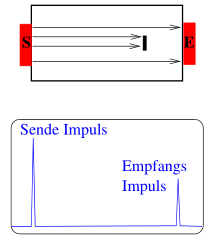
\includegraphics[width=0.3\textwidth]{latex/images/durchschall.PNG}
    \caption{Schematische Darstellung des Durchschallungs-Verfahrens und der Messdaten\protect \cite{US1}.}
    \label{img:durch}
\end{figure}

\noindent
Das erste Verfahren wird Durchschallungs-Verfahrens genannt.
Bei diesem Verfahren wird auf der einen Seite einer Probe ein Sender und auf der anderen ein Empfänger aufgebracht.
Falls sich zwischen den beiden eine Fehlstelle befindet lässt sich eine wesentliche Abnahme in der Intensität messen.
Eine Aussage über den genauen Ort lässt sich nicht schließen. 
Dieser Vorgang inklusive der schematischen Messwerte sind in Abbildung \ref{img:durch} dargestellt.

\begin{figure}[H]
    \centering
    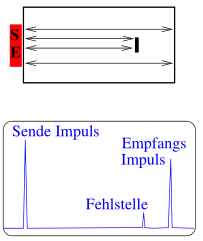
\includegraphics[width=0.3\textwidth]{latex/images/echo.PNG}
    \caption{Schematische Darstellung des Impuls-Echo-Verfahrens und der Messdaten\protect \cite{US1}.}
    \label{img:durch}
\end{figure}

\noindent 
Das zweite Verfahren ist das Impuls-Echo-Verfahren. 
Im Gegensatz zum Durchschallungs-Verfahren wird hier nur ein Sender aufgebracht, welcher auch als Empfänger dient.
Der ausgesendete Schallimpuls wird dabei teilweise von der Fehlstelle und vom Ende der Probe reflektiert. 
Über die Laufzeiten und Intensitäten lassen sich dann Rückschlüsse über den Ort und die Größe der Fehlstelle schließen.
Die Bestimmung des Ortes bei bekannter Schallgeschwindigkeit $c$ geht dabei über folgende Formel:
\begin{equation*}
    s=\frac{1}{2}c \cdot t
\end{equation*}
